\documentclass[a4paper,11pt]{article}
\usepackage{setspace}
\onehalfspacing
 
\usepackage{titlesec}
\usepackage{graphicx}
\usepackage{listings}
\usepackage{xcolor}
\usepackage{fancyhdr}
\usepackage[a4paper,margin=1in]{geometry}
\usepackage{mdframed} %nice frames

\definecolor{light-gray}{gray}{0.95} %the shade of grey that stack exchange uses

\renewcommand{\thispagestyle}[1]{} % do nothing

\lstset{
  language=Java,
  aboveskip=3mm,
  belowskip=3mm,
  showstringspaces=true,
  columns=flexible,
  basicstyle={\small\ttfamily},
  numbers=none,
  numberstyle=\tiny\color{gray},
  keywordstyle=\color{blue},
  commentstyle=\color{red},
  breaklines=true,
  breakatwhitespace=true,
  tabsize=2
}

\graphicspath{ {./images/} }
\titlespacing{\section}{0pc}{1pc}{1pc}
 
\pagestyle{fancy}
\fancyhf{}
\rhead{Tan Wei Xuan}
\lhead{Design \& Implementation: Internet Text Chatting Program}
\rfoot{Page \thepage}

 
\begin{document}
\title{\vspace{-1.0cm}\textbf{Design \& Implemenation: \linebreak Internet Text Chatting Program}}
\author{49003140 Tan Wei Xuan}
\date{\today}
\maketitle

\section{Project Overview}
The\textbf{ Internet Text Messaging Program} that I have implemented is a \textbf{Multi-threaded Chat Application} that utilises the Transmission Control Protocol \textit{(TCP)} and allows for mutiple clients to send/receive messages over a server, to one another, at the same time. My program is written in the \textit{\textbf{Java language}} and the source code files are as follow:
\begin{enumerate}
	\item \textbf{Server Files}
\begin{itemize}
  	\item ServerMain.java
 	\item Server.java.
\end{itemize}
	\item \textbf{Client Flients}
\begin{itemize}
  	\item Client.java
 	\item ClientThread.java
\end{itemize}
\end{enumerate}

\section{Design}
My program is built on the  \textit{Java Socket Programming API} and the transfer protocol used is the \textbf{Transmission Control Protocol \textit{(TCP)}}.
I have chosen to use \textbf{TCP} instead of \textbf{User Datagram Protocol \textit{(UDP)}} as my transfer protocol as TCP outweighs UDP in terms of reliablity and it has in-order data delivery.There are 4 tuples in a TCP connection and there are as follow:
\begin{enumerate}
  \item Source IP Address
  \item Source Port
  \item Target IP Address
  \item Target Port
\end{enumerate}

\noindent My program utilises the \textbf{Sockets API Library} for Java, \textit{java.net.ServerSocket} and  \textit{java.net.Socket}, to implement the Socket Client and Socket.\textit{ java.net.ServerSocket} provides a system-independent implementation of the server side of a client/server socket connection.\textit{ java.net.Socket} implements client sockets and the socket is an endpoint for communication between two machines.The design of my program is based on the sequence of socket API calls and client/server communication flow for TCP (shown below).

\begin{figure}[h!]
\begin{center}
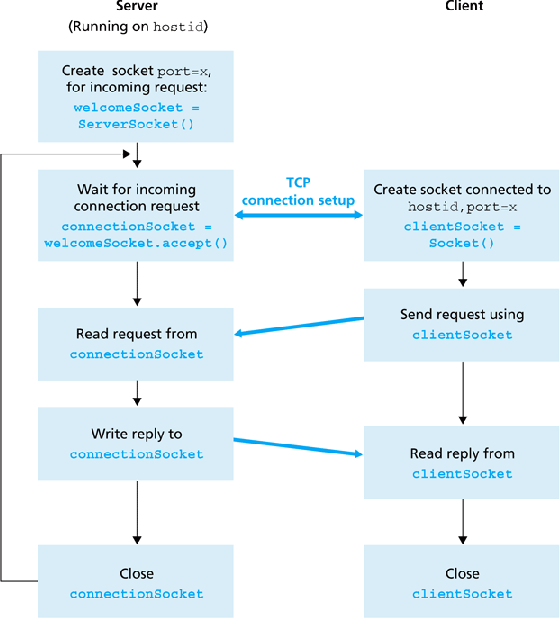
\includegraphics[scale=0.5]{socketflow}
\caption{''TCP Client/Server Communication Flow''} 
\end{center}
\end{figure}

\section{Implementation}
\subsection{Server}
The server utilises the \textit{ServerSocket} class to implement the server side of the client/server socket connection.
Usually, a server runs on a specific computer on the network and has a socket that is bound to a specific port number and a Host name \textit{(IP-to-Host name resolution)} obtainable through the\textit{InetAddress class}. In my project, we use the same computer as both the client and the server. 
\subsection{Client}
The Client utilises the \textit{Socket} class to implement the client side of the client/server socket connection. The client must know the hostname or IP of the machine on which the server is running and the port number on which the server is listening. In my project, the port I am using is \textit{2222} and the hostname is  \textit{localhost}

\subsection{Client Thread}
The Client Thread is a \textbf{thread} utilised by the Server to service multiple Clients simultaneously by allowing multiple clients to be connected to the server concurrently and creating  a new socket for every new client. It services each client's request different thread. The number of clients being served simultaneously will equal the number of threads running. The Client thread reads from and writes to the client connection as necessary.

\section{Client/Server Communication Flow Implementation}

\subsection{Create Server Socket port}
My program begins by creating a new \textit{ServerSocket} object to listen on a specific port. When running this server, choose a port that is not already dedicated to some other service. In my program, the server is started on port \textit{2222} with \textit{localhost} as the \textit{Host Name}.
\begin{mdframed}[backgroundcolor=light-gray, roundcorner=30pt,leftmargin=1, rightmargin=1, innerleftmargin=5, innertopmargin=-3,innerbottommargin=5, outerlinewidth=1, linecolor=light-gray]
\begin{lstlisting}
//ServerMain.java
//Port number can be changed
final int portNumber = 2222;
//IP-to-Host Name Resolution
//Can be configured to connect to external IP address
final InetAddress addr = InetAddress.getByName("127.0.0.1");
\end{lstlisting}
\end{mdframed}

\begin{mdframed}[backgroundcolor=light-gray, roundcorner=30pt,leftmargin=1, rightmargin=1, innerleftmargin=5, innertopmargin=-3,innerbottommargin=5, outerlinewidth=1, linecolor=light-gray]
\begin{lstlisting}
//Server.java
//Open a Server Socket on the Port Number
serverSocket = new ServerSocket(serverPort,0,addr);
\end{lstlisting}
\end{mdframed}

\subsection{Wait for Incoming Connection Request}
If the server successfully binds to its port, then the \textit{ServerSocket} object is successfully created and the server continues to the next step - accepting a connection from a client .The accept method waits until a client starts up and requests a connection on the host and port of this server. 
\begin{mdframed}[backgroundcolor=light-gray, roundcorner=30pt,leftmargin=1, rightmargin=1, innerleftmargin=5, innertopmargin=-3,innerbottommargin=5, outerlinewidth=1, linecolor=light-gray]
\begin{lstlisting}
//Server.java
Socket clientSocket = serverSocket.accept();
\end{lstlisting}
\end{mdframed}

\subsection{Create Client Socket connecting to Server}
The server should already be running and listening to the port, waiting for a client to request a connection. The first thing the client program does is to open a socket that is connected to the server running on the specified host name and port:
\begin{mdframed}[backgroundcolor=light-gray, roundcorner=30pt,leftmargin=1, rightmargin=1, innerleftmargin=5, innertopmargin=-3,innerbottommargin=5, outerlinewidth=1, linecolor=light-gray]
\begin{lstlisting}
//Client.java
// The client socket
private static Socket clientSocket = null;
// The output stream
// The server port.
int portNumber = 2222;
// The server host.
// For now we are using localhost
String host = "localhost";
clientSocket = new Socket(host, portNumber);
\end{lstlisting}
\end{mdframed}

\subsection{Server - Write/Receive message from Client}
At this point, the new Socket object puts the server in direct connection with the clientl, allowing us to access the output and input streams to write and receive messages to and from the client respectively. The server is capable of exchanging messages with the client endlessly until the socket is closed with its streams.
\begin{mdframed}[backgroundcolor=light-gray, roundcorner=30pt,leftmargin=1, rightmargin=1, innerleftmargin=5, innertopmargin=-3,innerbottommargin=5, outerlinewidth=1, linecolor=light-gray]
\begin{lstlisting}
//ClientThread.java
//For Receiving Messages from Client
inputStream = new DataInputStream(clientSocket.getInputStream());
//For Writing Message to Client
outputStream = new PrintStream(clientSocket.getOutputStream());
\end{lstlisting}
\end{mdframed}

\subsection{Client - Write/Receive message from Server}
When the server has accepted the connection, we can then obtain input and output streams from the \textit{Client Socket} to communicate with the server. The input stream of the client is connected to the output stream of the server, just like the input stream of the server is connected to the output stream of the client.
\begin{mdframed}[backgroundcolor=light-gray, roundcorner=30pt,leftmargin=1, rightmargin=1, innerleftmargin=5, innertopmargin=-3,innerbottommargin=5, outerlinewidth=1, linecolor=light-gray]
\begin{lstlisting}
//Client.java
//Output Stream is connected to the Input Stream of the server
outputStream = new PrintStream(clientSocket.getOutputStream());
//Input Stream is connected to the Output Stream of the server
inputStream = new DataInputStream(clientSocket.getInputStream());
\end{lstlisting}
\end{mdframed}

\subsection{Client - Closing Connection}
In my program, stopping the connection to the server is done when the client input the word, \textit{"/quit"}. By doing this, alll the Client's Input and Output Streams and the Client's socket will be closed 
\begin{mdframed}[backgroundcolor=light-gray, roundcorner=30pt,leftmargin=1, rightmargin=1, innerleftmargin=5, innertopmargin=-3,innerbottommargin=5, outerlinewidth=1, linecolor=light-gray]
\begin{lstlisting}
//ClientThread.java
while (true) {
	String line = inputStream.readLine();
	if (line.length() <= 0)
	continue;
	//Quits the chatroom
	else if (line.startsWith("/quit")) {
		break;
	}
}
//Closes the Input/Output Stream and the Client Socket
inputStream.close();
outputStream.close();
clientSocket.close();
\end{lstlisting}
\end{mdframed}

\subsection{Server - Closing Connection}
As my program is a multi-threaded chat server where multiple clients will be able to connect/disconnect at any time as long as the server is open, closing off the server will require the \textit{host} to close off the \textit{Server Socket} explictly on his/her end. This will release the port that the server is being binded to and prevent any more clients from connecting to it. The server can be terminated through either the \textit{command prompt/terminal} or the \textit{Integrated Development Environment (IDE)}.

\section{Running the Program}
\subsection{Integrated Development Environment}
\begin{enumerate}
  \item Import the Project
  \item Run \textbf{\textit{ServerMain.java}} to start the \textbf{server}  
  \item  Run \textbf{\textit{Client.java}} to start the client (Run \textit{\textbf{n}} times to start \textit{\textbf{n}} clients)
\end{enumerate}
\subsection{Exectuables}
\begin{enumerate}
  \item Run \textbf{\textit{ServerMain.bat}} to start the \textbf{server}\textit{(*DO NOT run SeverMain.jar)}
  \item  Run \textbf{\textit{Client.jar}} to start the client (Run \textit{\textbf{n}} times to start \textit{\textbf{n}} clients)
\end{enumerate}
\section{References}
\noindent [1] A Guide to Java Sockets
\newline
\underline{https://www.baeldung.com/a-guide-to-java-sockets}
\newline
\newline
[2] Writing the Server Side of a Socket
\newline
\underline{https://docs.oracle.com/javase/tutorial/networking/sockets/clientServer.html}
\newline
\newline
[3] Java Socket Programming - Socket Server, Client Example
\newline
\underline{https://www.journaldev.com/741/java-socket-programming-server-client}
\end{document}